\chapter[Conclusions and Future Work]{Conclusion and Future Work}
\chaptermark{Conclusions and Future Work}
\label{chap:conclusion}
\minitoc

\newpage

In this section, we will highlight some of the major contributions that were achieved within this thesis. We will further discuss the major shortcomings as well as future prospectives that could address those limitations. 

\section{Summary}
In the introductory \chapref{chap:introduction}, we analyzed the inevitable rise of robot assisted laparoscopy and linked it to surgeon benefits and future prospects, \secref{in:sec:the_rise_of_robot_assisted_laparoscopy}. We identified spatial awareness and automation as key targets for enhancing and alleviating, driving factors and roadblocks, respectively, see \figref{in:fig:advancing_robotic_laparoscopy}. To address these, we proposed marker-free unified calibration for enhanced spatial awareness with improved clinical workflow in \secref{in:sec:marker_free_unified_calibration}. Moreover, in \figref{in:fig:hypothesized_pipeline}, we outlined a framework for learning to imitate camera motion from a camera-assistant-held laparoscope, see \figref{in:fig:room_setup}. We argued that, through a mixture of classical control, and imitation learning in image space, it might be possible to imitate a surgeon through a robot laparoscope holder despite their different embodiment. The following sections will discuss the extend to which the proposed solutions met the pinpointed targets, and further suggest future research directions when targets where not fully met or could improved upon.

\section{Marker-free Unified Eye-hand Calibration}
\label{con:sec:marker_free}

\chapref{chap:registration}

\begin{figure}
    \centering
    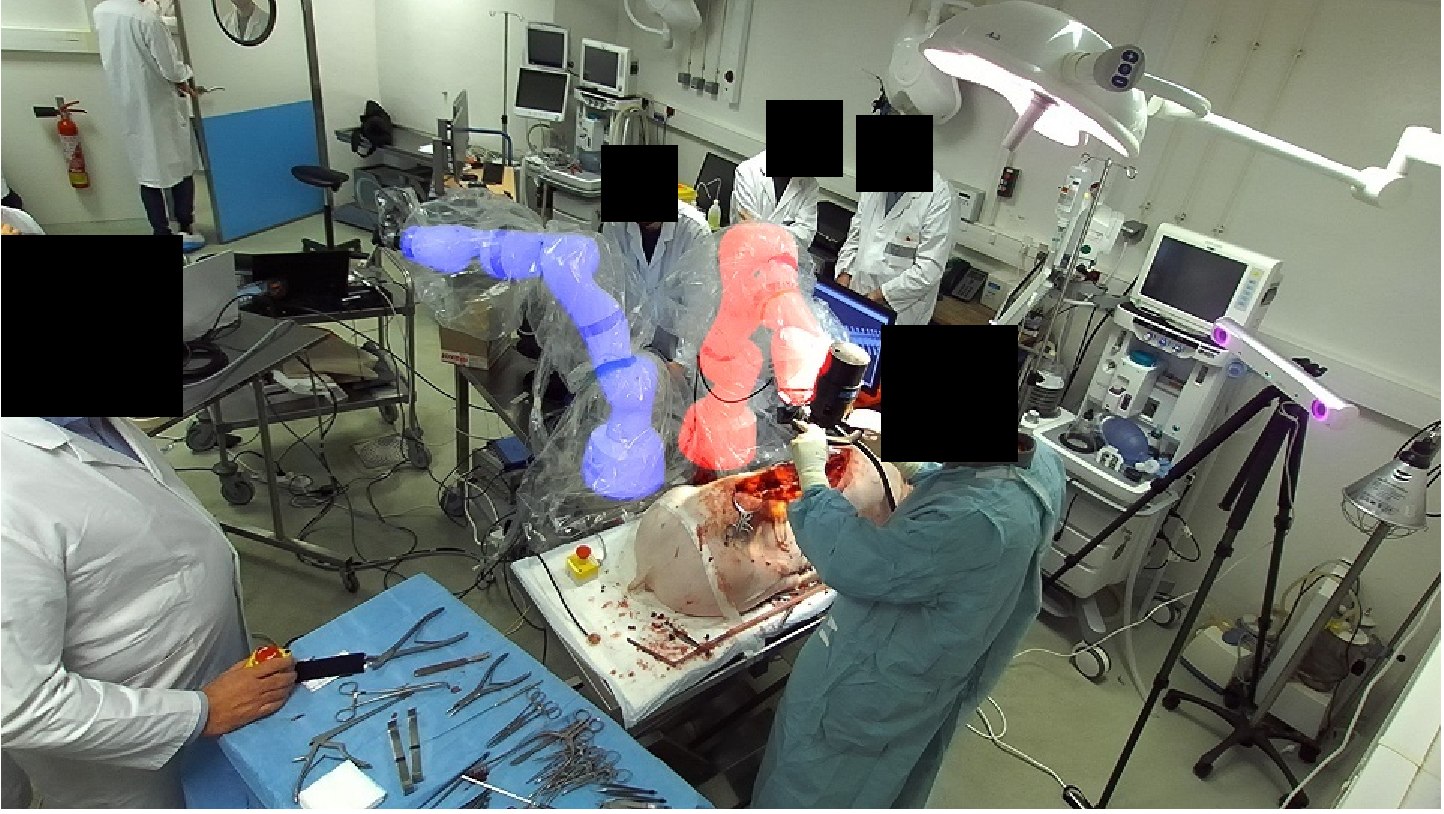
\includegraphics[width=\textwidth]{conclusion/img/draped_ground_truth.pdf}
    \caption{Caption. Refers to \secref{con:sec:marker_free}.}
    \label{con:fig:draped_ground_truth}
\end{figure}
- less dependencies, test of time
- differentiable rendering -> solving draped robots

\section{Homography-based Visual Servo with Remote Center of Motion Constraint}
\label{con:sec:visual_servo}
\paragraph{Contributions} In \chapref{chap:robotic_endoscope}, we introduced a novel image-based visual servoing approach with RCM constraint. We attempted to shift the control paradigm from a tool-centric control policy towards a view-centric control policy to address the flaws of the dominant visual servos, refer \secref{in:sec:rule_based_approaches}, \figref{in:fig:com}. To this end, we derived a homography-based visual servo which does not rely on depth nor on tool distance for inferring actions \figref{c2:fig:schematic}. We did so, introducing a projection operator for mapping target camera frame velocities to available DOF, \eqref{c2:eq:proj}. We then deployed the newly derived control in a novel view-graph-based semi-autonomous scheme on a real system, see \figref{c2:fig:pipe}, \figref{in:fig:experimental_setup}. The proposed method demonstrated good image space convergence properties throughout traversing the view graph from current to target view whilst retained a deviation from the target RCM below $5\,\text{mm}$, see \figref{c2:fig:errors}. The proposed method further indicated robustness against patient re-positioning, i.e. coordinate system change, see \tabref{c2:tab:repositioning}.

\paragraph{Shortcomings and Future Work} The most apparent shortcoming of the proposed method is the assumption of a mostly static surgical scene which clearly does not hold, see \figref{c2:fig:tool_insertion_trajectory}. This temporality assumption, however, is not so crucial within the overarching context of the thesis, as ultimately the executed action is not graph-based but rather incrementally sampled from a learned expert policy $\pi_\text{E}:\, \hat{s}_t \rightarrow \hat{a}^*_t$, refer \secref{in:sec:imitation_learning}. A shortcoming that weighs much heavier is e.g. the lack of force sensing. No trocar-laparoscope external forces nor arm-environment external forces are incorporated into the controller. Arm-environment external forces could e.g. be minimized through nullspace projection and the redundant DOF of the manipulator. The proposed controller furthermore does not explicitly constrain solutions to the RCM, and convergence to undesired minima might occur. Further research should thus introduce constrained optimization instead.

\paragraph{Take-away} Altogether, it was demonstrated that indeed the introduced visual servo could serve as means for executing actions $\hat{a}^*_t$ for the hypothesized pipeline, refer \figref{in:fig:hypothesized_pipeline}, but that future improvements would be necessary for successful clinical translation.

\section{Homography-based Camera Motion Estimation}
\label{con:sec:hom_est}

\chapref{chap:camera_motion_extraction}
- novel view synthesis
    - runtime for data
    - no diffusion models \cite{rombach2022high} as these tend to hallucinate and iterative  
\begin{figure}
    \centering
    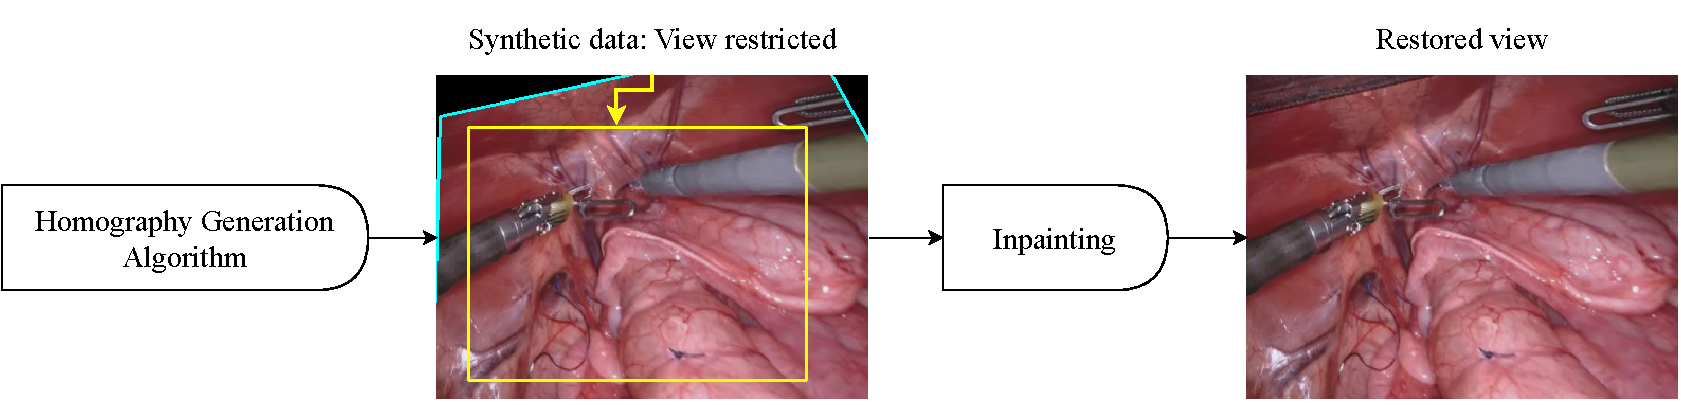
\includegraphics[width=\textwidth]{conclusion/fig/fourier_inpainting.pdf}
    \caption{Algorithm from \secref{c3:sec:hom_gen} \figref{c3:fig:hom} Caption \cite{suvorov2021resolution}. Refers to \secref{con:sec:hom_est}.}
    \label{con:fig:inpainting}
\end{figure}
- incorporate depth \cite{budd2024transferring}: novel view synthesis
- utilize inpainting methods as well
- inpainting -> better range


\section{Homography-based Camera Motion Prediction}
\label{con:sec:hom_pred}

\chapref{chap:camera_motion_prediction}

- rl on-top (force controlled rcm, rlhf)
- bootstrapping motion:
    - visual qa
- llm interface models: \figref{in:fig:hypothesized_pipeline} (beyond scope)


\section{Final Words}
the proposed pipeline holds an interesting framework for self-supervised .... indeed proving that \figref{in:fig:auxiliary_tasks}
